We will measure now the execution time of our solution, that we called \textbf{bwa-gasal2}, and compare it to the mainline version of BWA. For all this section, bwa-gasal2 processes sequences in batches of 1000, which gives between 10 000 and 100 000 chains to process for each batch.

\subsection{Data set SRR150}

For the first data set, full program execution times are given on figure \ref{fig:total-exec-time-srr150} and kernel speed-ups against BWA on figure \ref{fig:total-exec-speed-up-srr150}. We can notice that the global speed-up fluctuates quite a lot when using different threads, but no trend can be inferred. This may be due to our testing conditions or simply due to the nature of the data set, the results may present uneven behaviour depending on how data is split between threads.

\begin{figure}[p]
	\centering
	\begin{subfigure}[t]{1\textwidth}
		\centering
			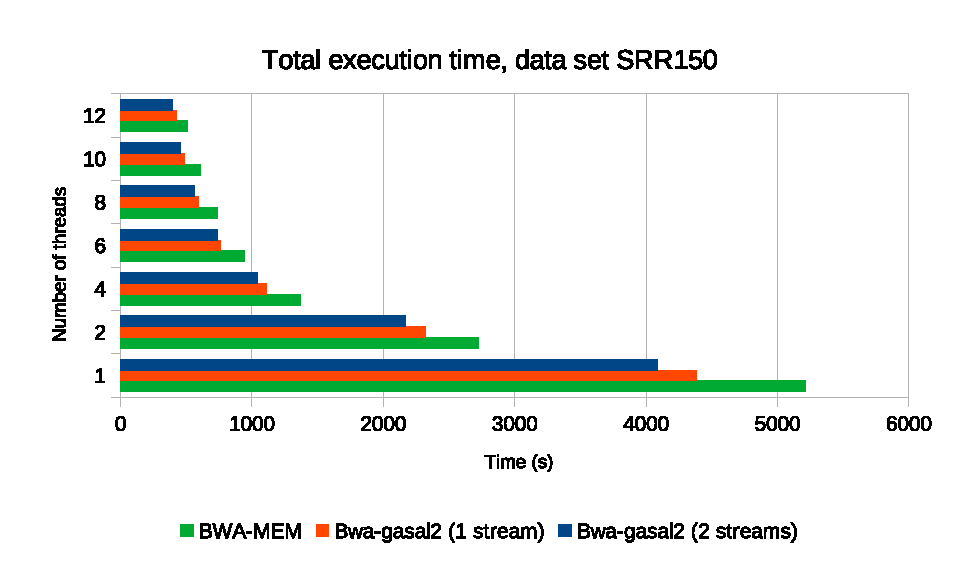
\includegraphics[width=1\textwidth]{srr150/total-exec-time-srr150}
		\caption{Total execution time for SSR150}
		\label{fig:total-exec-time-srr150}
	\end{subfigure}%
	
	\begin{subfigure}[b]{1\textwidth}
		\centering
		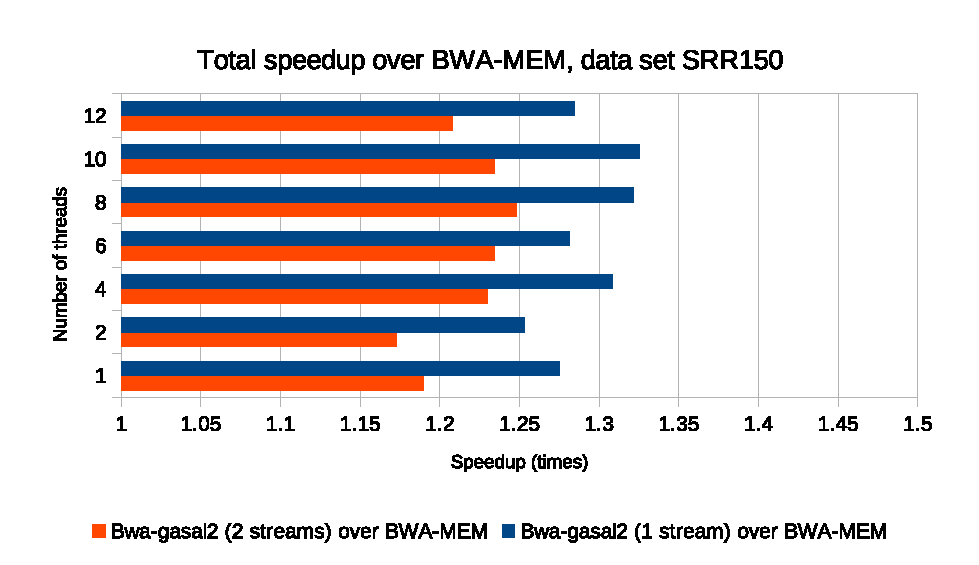
\includegraphics[width=1\textwidth]{srr150/total-exec-speed-up-srr150}
		\caption{Speed-up for the whole program execution for SRR150}
		\label{fig:total-exec-speed-up-srr150}
	\end{subfigure}
	\caption{Program results for data set SRR150}
	%\label{fig:}
\end{figure}


We obtain the most important speed-up using a single thread, reaching 1.35$\times$ the original program speed. This is promising, but is hardly a good indicator: in fact, these kind of program is usually run with multiple threads, and as we mentioned on chapter \ref{chap:accel}, a single thread running the accelerator is far from sufficient to saturate the GPU computing resources.

In the case of 12 threads, we reach a GPU occupation of around 95\%, which is the kind of figure we are looking for. Here, the total speed-up almost reaches 1.28$\times$. It is substantially below our theoretical maximum of 1.37$\times$, but we are getting closer. Many factors can participate in making this difference. In particular, memory filling for the batches requires a significant amount of time on the CPU side, in addition to the memory copies from host to device. In this case, we started with an already large memory allocation, to avoid any overhead caused by new allocations.

In all cases, the difference between one and two streams is striking, with the speed-up even leaping from 1.21$\times$ to 1.28$\times$ in the 12 threads case.

When isolating the kernel times and kernel speed-up, we get the measurements shown respectively on figure \ref{fig:kernel-exec-time-srr150} and figure \ref{fig:kernel-exec-speed-up-srr150}. It is important to notice that what is reported as "kernel time" for the 2-stream variant represents the time during which the CPU is actively waiting for the GPU results. In other words, we have hidden-time execution disabled when using one stream, and enabled with 2 streams. We call this "visible kernel execution time".


\begin{figure}[p]
	\centering
	\begin{subfigure}[t]{1\textwidth}
		\centering
		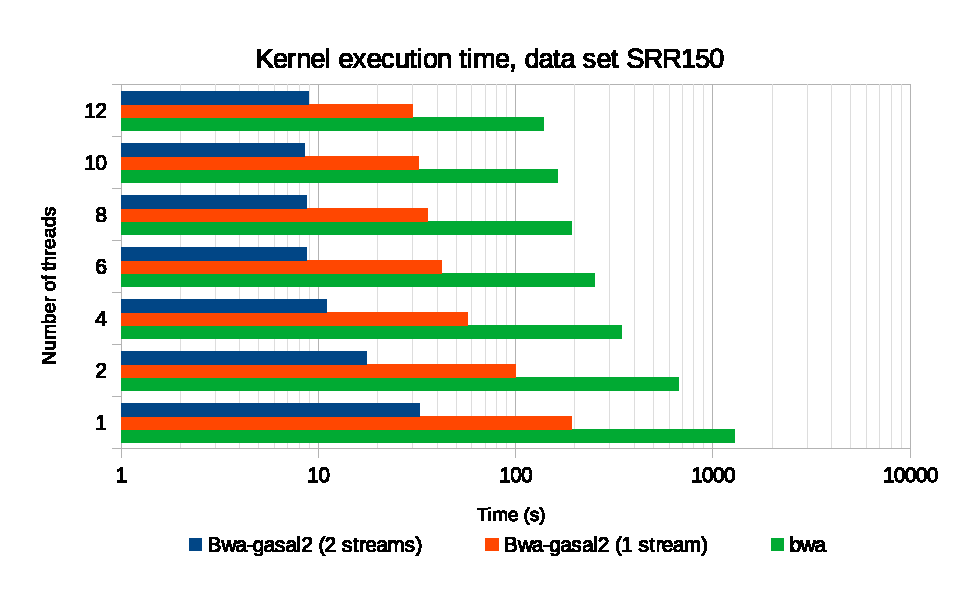
\includegraphics[width=1\textwidth]{srr150/kernel-exec-time-srr150}
		\caption{Visible kernel execution time for SRR150}
		\label{fig:kernel-exec-time-srr150}
	\end{subfigure}%
	
	\begin{subfigure}[b]{1\textwidth}
		\centering
		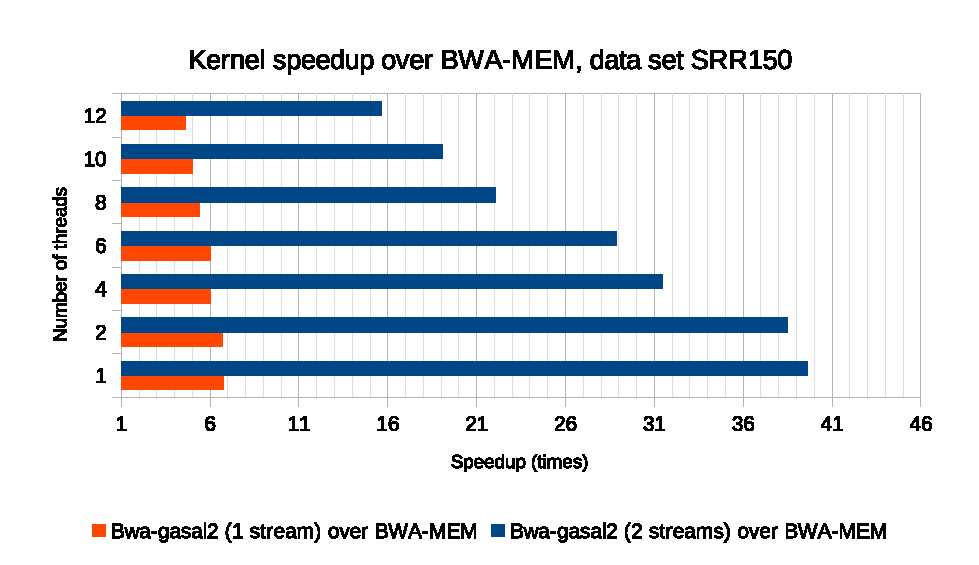
\includegraphics[width=1\textwidth]{srr150/kernel-exec-speed-up-srr150}
		\caption{Speed-up for the kernel execution for SRR150}
		\label{fig:kernel-exec-speed-up-srr150}
	\end{subfigure}
	\caption{Kernel results for data set SRR150}
	%\label{fig:}
\end{figure}

With hidden-time execution, on the 2-stream version, the visible kernel time is simply an order of magnitude shorter. In this special case, the kernel times were hugely different, so we had to display them in log scale. But while the visible sped-up reaches 4.7$\times$ on single streams with 12 threads, it jumps to almost 16$\times$, effectively shrinking down the visible compute time of the extension by the same amount. Although it is not useful in real-life, single-thread results are even more impressive, with a visible kernel speed-up reaching 40$\times$ with hidden-time, and only 6$\times$ when actively waiting for the result.


\subsection{Data set SRR250}

We run the same measurements on data set SRR250. Its sequences are longer, so they take quite a substantial amount of time to complete. Execution times and overall speed-up are shown on figure \ref{fig:total-exec-time-srr250} and figure \ref{fig:total-exec-speed-up-srr250} respectively.


\begin{figure}[p]
	\centering
	\begin{subfigure}[t]{1\textwidth}
		\centering
		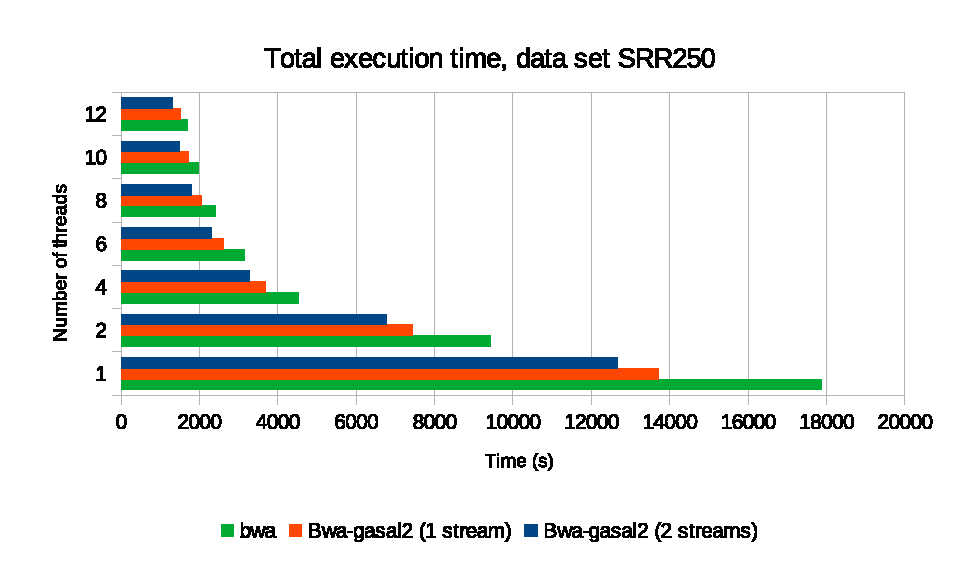
\includegraphics[width=1\textwidth]{srr250/total-exec-time-srr250}
		\caption{Total execution time for SSR250}
		\label{fig:total-exec-time-srr250}
	\end{subfigure}%
	
	\begin{subfigure}[b]{1\textwidth}
		\centering
		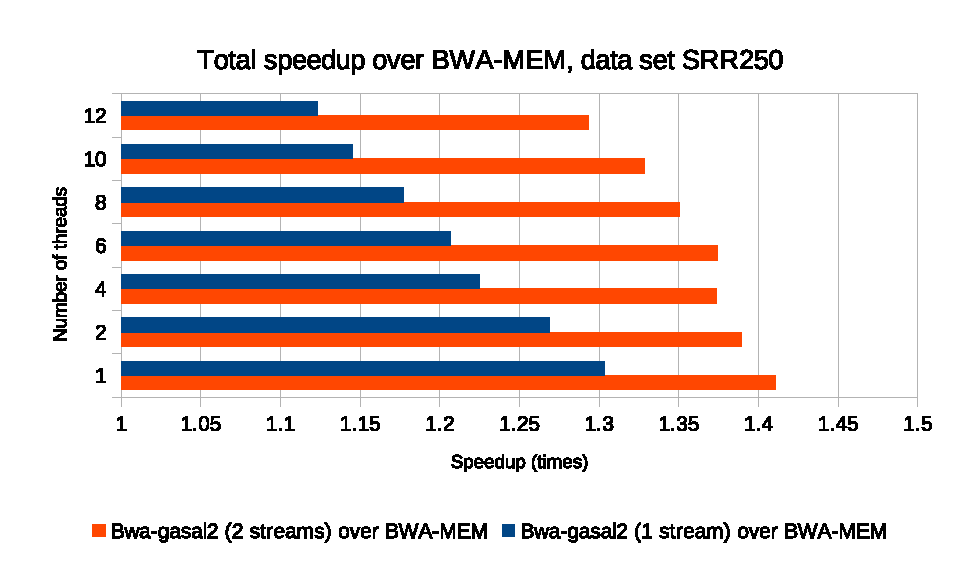
\includegraphics[width=1\textwidth]{srr250/total-exec-speed-up-srr250}
		\caption{Speed-up for the whole program execution for SRR250}
		\label{fig:total-exec-speed-up-srr250}
	\end{subfigure}
	\caption{Program results for data set SRR250}
	%\label{fig:}
\end{figure}

For this data set, the extension time is taking approximately 33\% of the total time, so we would expect a bigger speed-up, with the theoretical maximum being 1.5$\times$. However, it is not what we observe, even in the best case with 2 streams: on a single thread, we can effectively reach a speed-up of 1.41$\times$, which gets somewhat close to the theoretical maximum, but with 12 threads, we reach only 1.29$\times$. This is still a valuable improvement over the original version, and in all cases, hidden-time execution gives a substantial boost in performance. When comparing the single stream version to its 2-stream counterpart, we note that using 2 streams definitely helps shrinking the execution time.

Let's examine the kernel times and speed-up, on figure \ref{fig:kernel-exec-time-srr250} and \ref{fig:kernel-exec-speed-up-srr250} respectively.


\begin{figure}[p]
	\centering
	\begin{subfigure}[t]{1\textwidth}
		\centering
		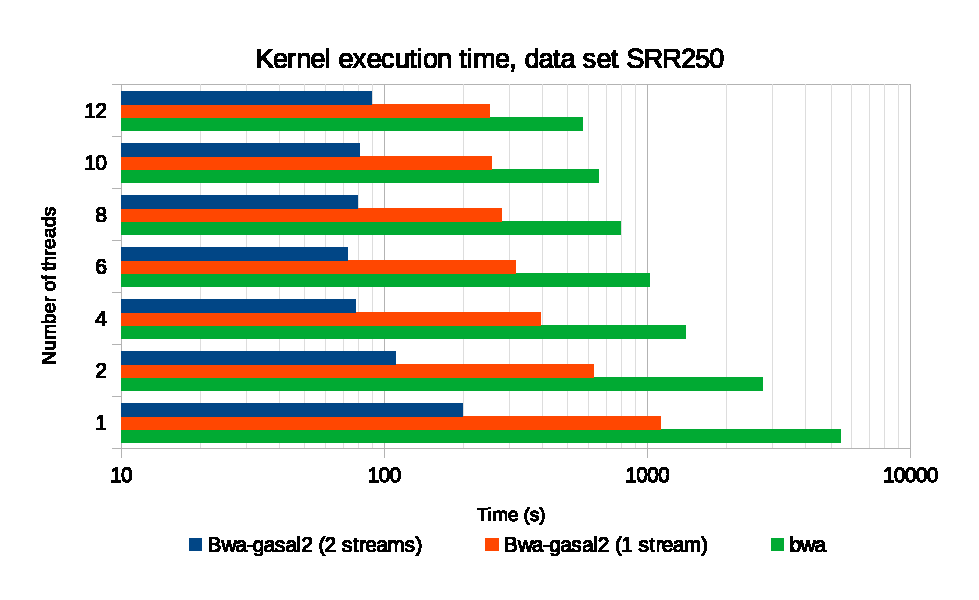
\includegraphics[width=1\textwidth]{srr250/kernel-exec-time-srr250}
		\caption{Visible kernel execution time for SRR250}
		\label{fig:kernel-exec-time-srr250}
	\end{subfigure}%
	
	\begin{subfigure}[b]{1\textwidth}
		\centering
		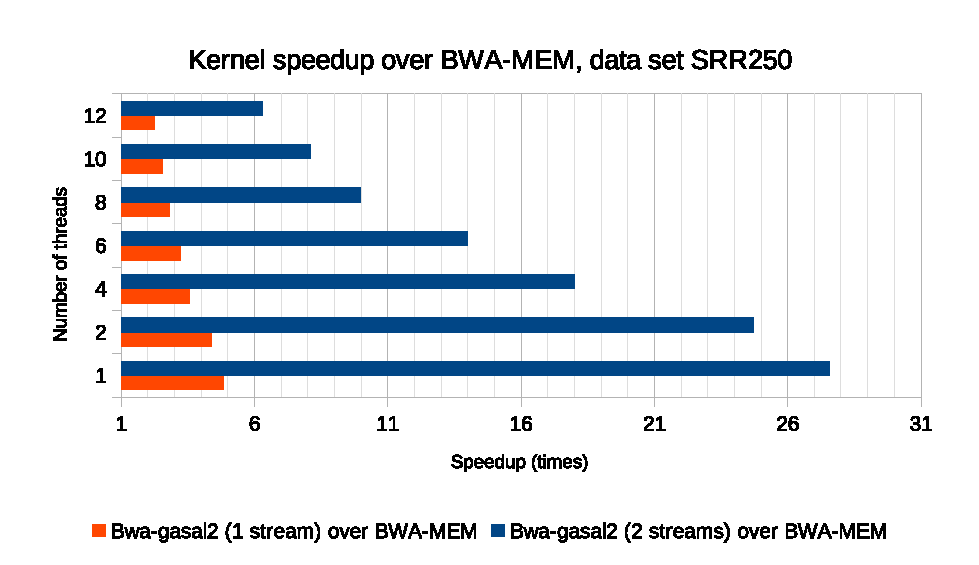
\includegraphics[width=1\textwidth]{srr250/kernel-exec-speed-up-srr250}
		\caption{Speed-up for the kernel execution for SRR250}
		\label{fig:kernel-exec-speed-up-srr250}
	\end{subfigure}
	\caption{Visible kernel execution for data set SRR250}
	%\label{fig:}
\end{figure}

Kernel running times for BWA (running on CPU) are somewhat steady. As the number of threads increases, we get closer to a plateau as the execution time hardly gets any lower for all programs. Again, we can remark how hidden-time execution helps in computing it faster with two streams. The difference is tremendously high for one thread, with time the CPU waiting for the GPU to complete being 5 times lower with 2 streams (from 1125s with 1 stream to 197s), but the benefits are not as high when using 12 threads, with the kernel waiting time being only 2.5 lower for the 2-stream version (from 250s for 1 stream to 89s for 2 streams). When using multiple threads, the overhead caused by filling a lot of GPU batches then copying them to the device is more important. It is all the more the case when using twice as many streams, having twice as many structures needing filling and being copied to the device.

We can also see whether increasing the number of streams could give any performance improvement. Results are shown on figure \ref{fig:exec-time-nbstreams}. As we can see, more than 2 streams does not result in any improvement. 

\begin{figure}[h]
	\centering
	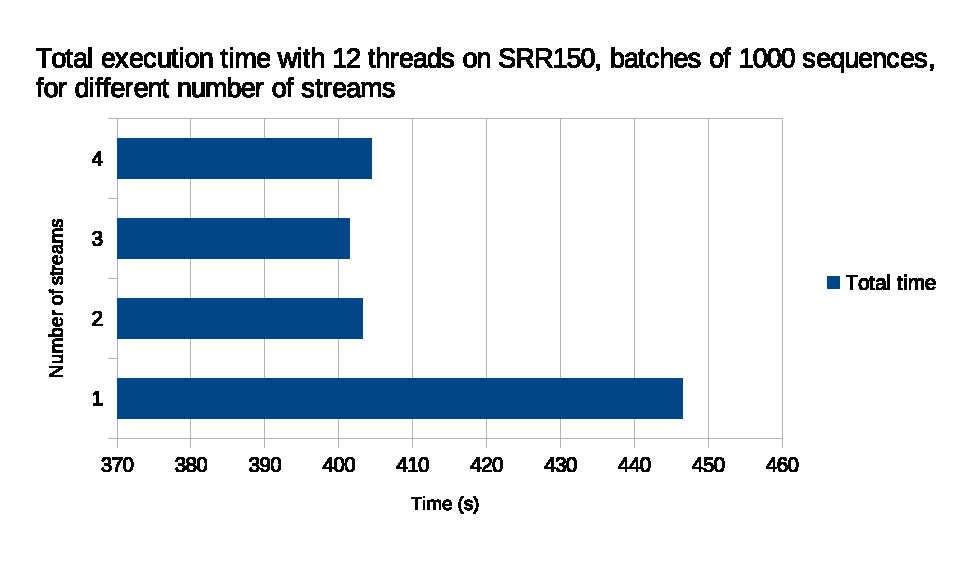
\includegraphics[width=0.9\linewidth]{exec-time-nbstreams}
	\caption{Execution time for 12 threads and different number of streams, data set SRR150}
	\label{fig:exec-time-nbstreams}
\end{figure}

% Note: this newpage is nice here, but depending on the content above, it may be ugly.
% \newpage